\begin{figure}[H]
	\centering
	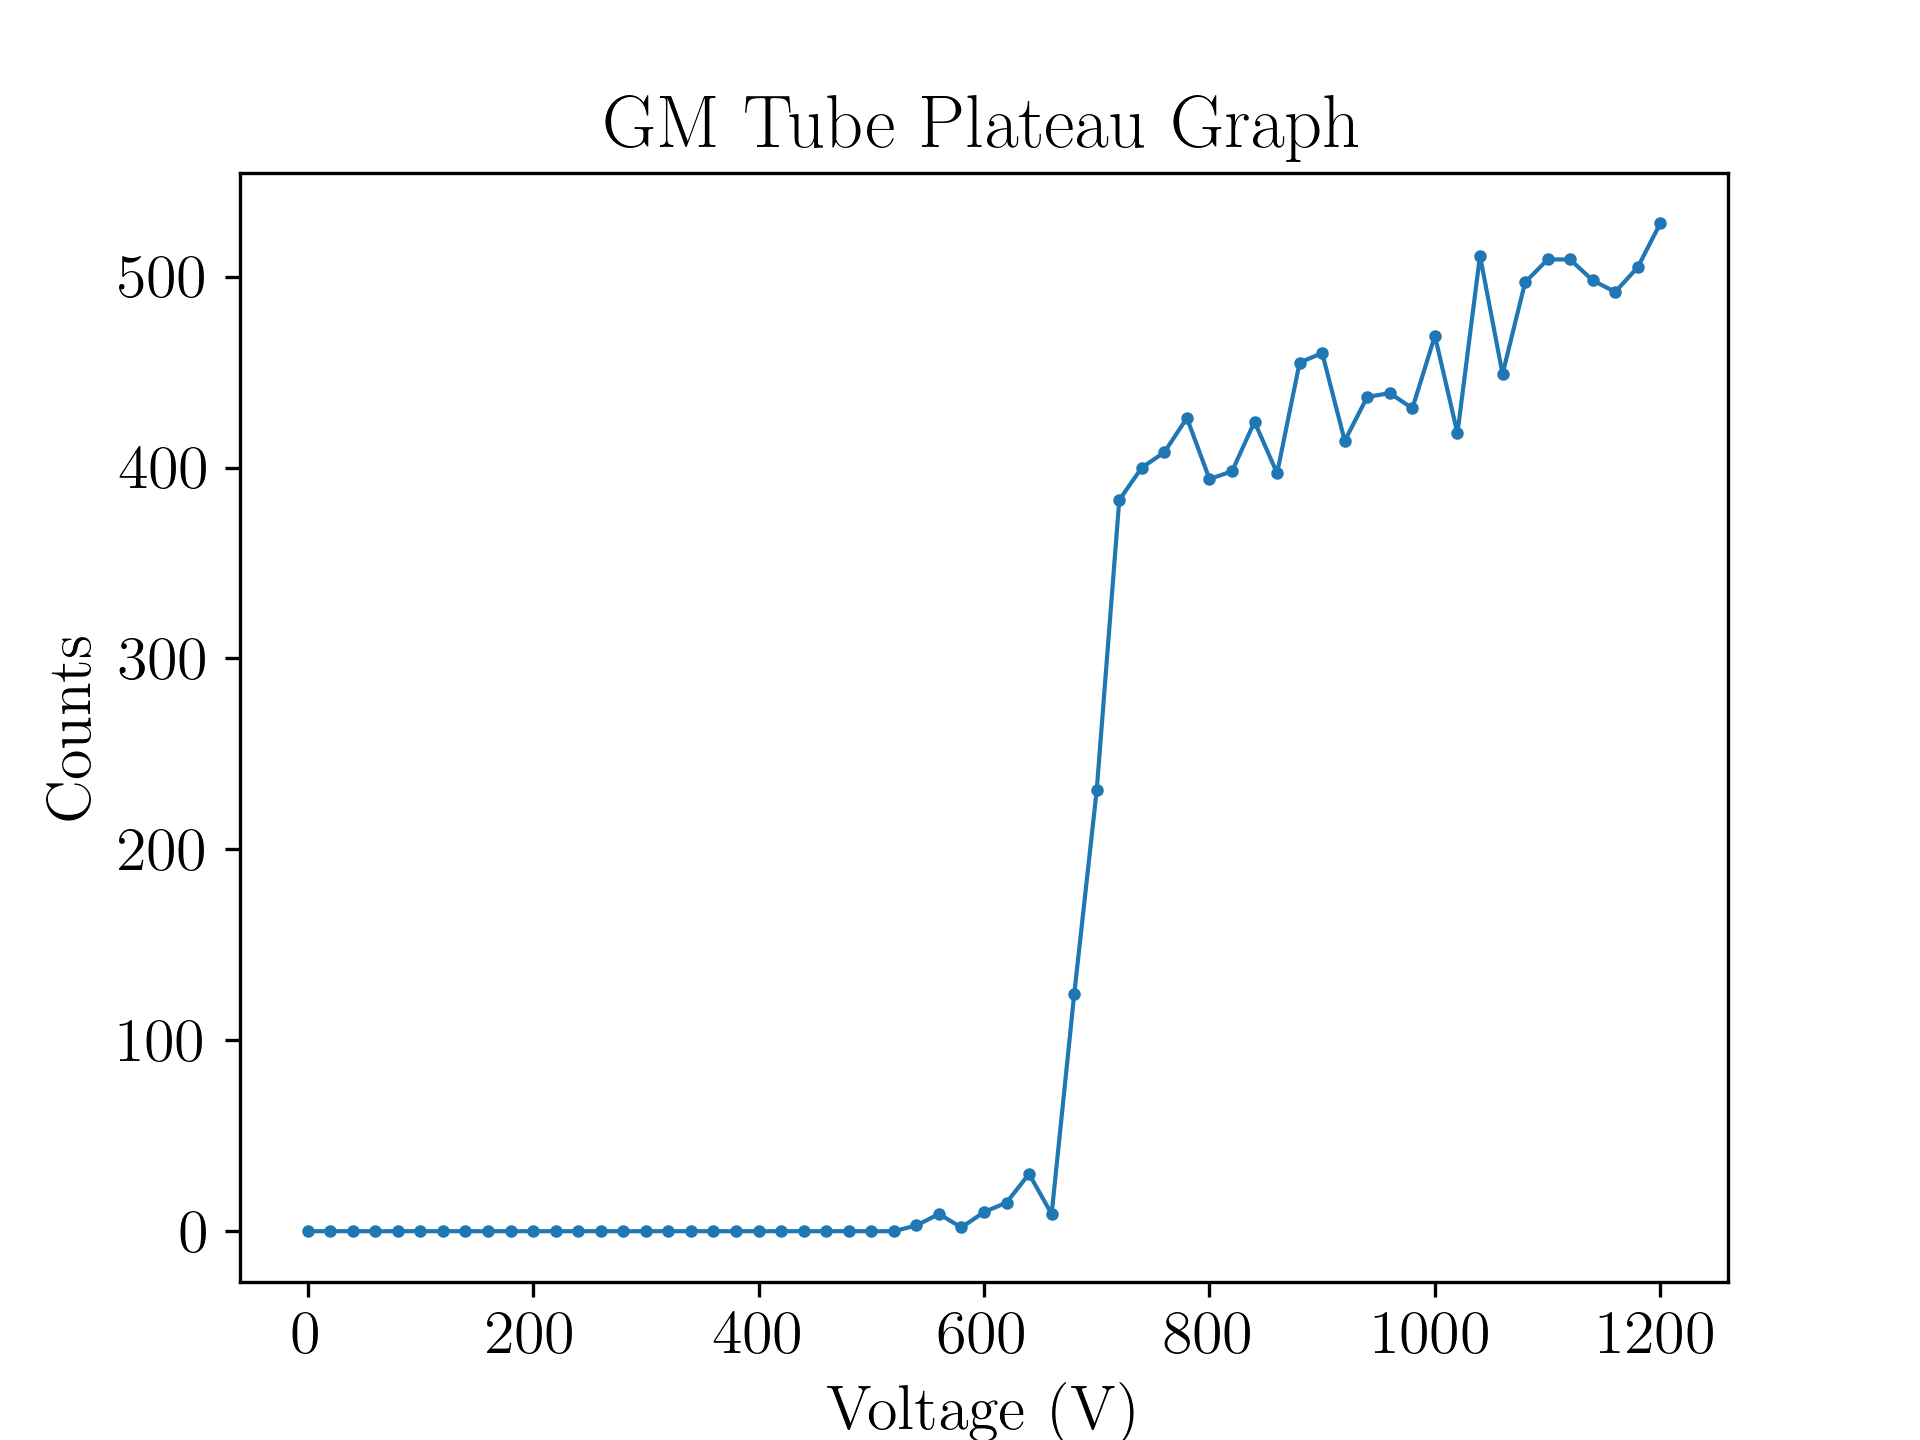
\includegraphics[scale=1]{PlateauGraph.png}
	\caption{Counts vs. Voltage (V) for the plateau curve experiment, where the operating voltage of the Geiger-Muller tube was increased by 20 V from 0 V to 1200 V.}
\end{figure}

\begin{figure}[H]
	\centering
	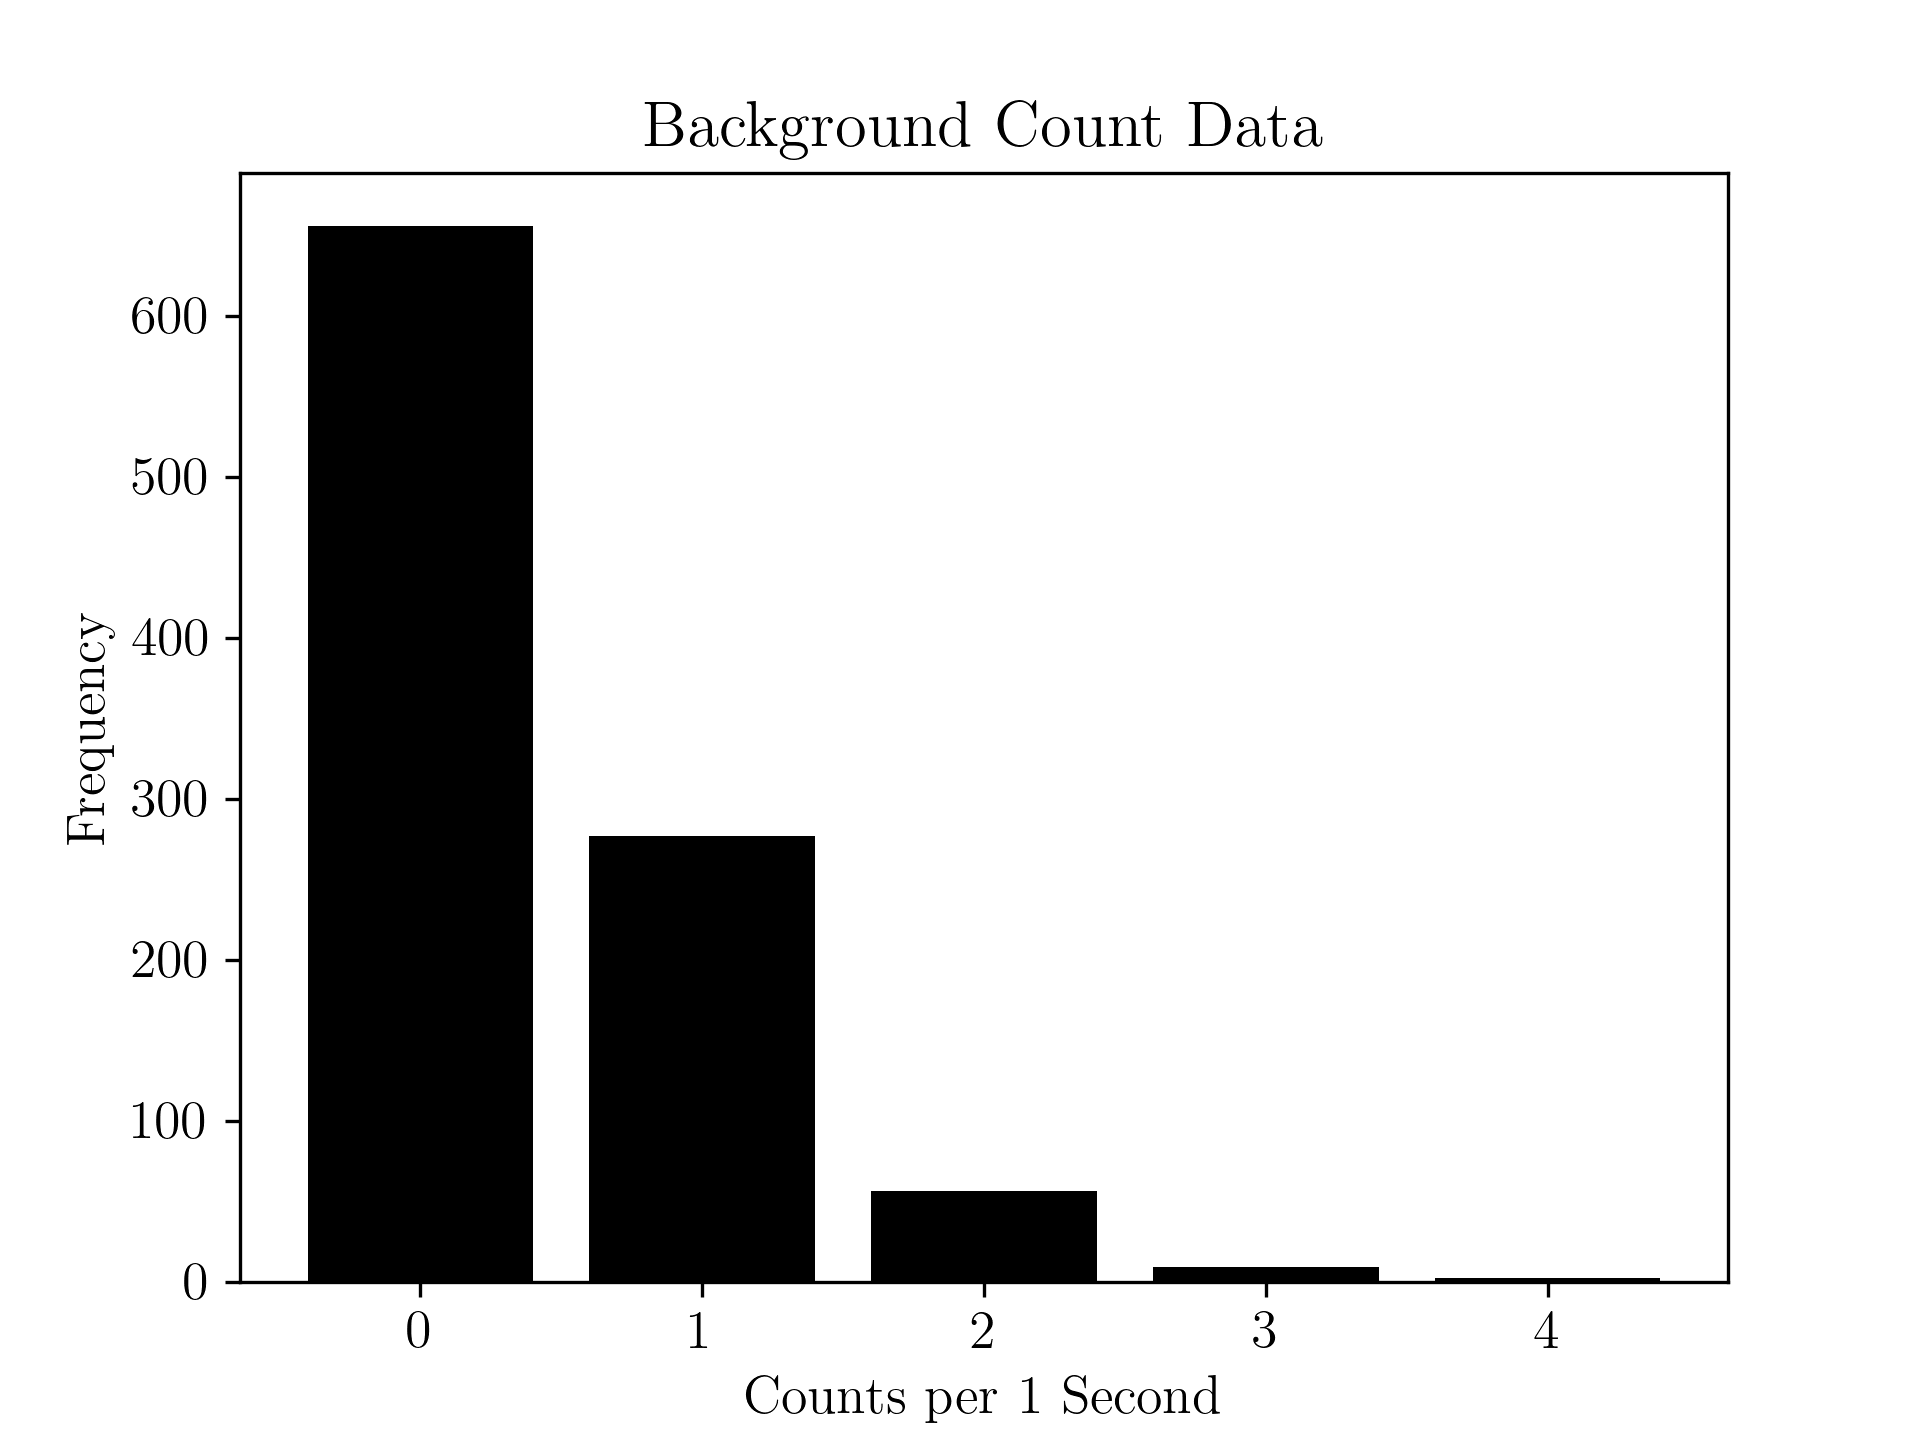
\includegraphics[scale=1]{BackgroundCountHist1sec.png}
	\caption{Count distributions over intervals of 1 second for the background measurement.}
\end{figure}

\begin{figure}[H]
	\centering
	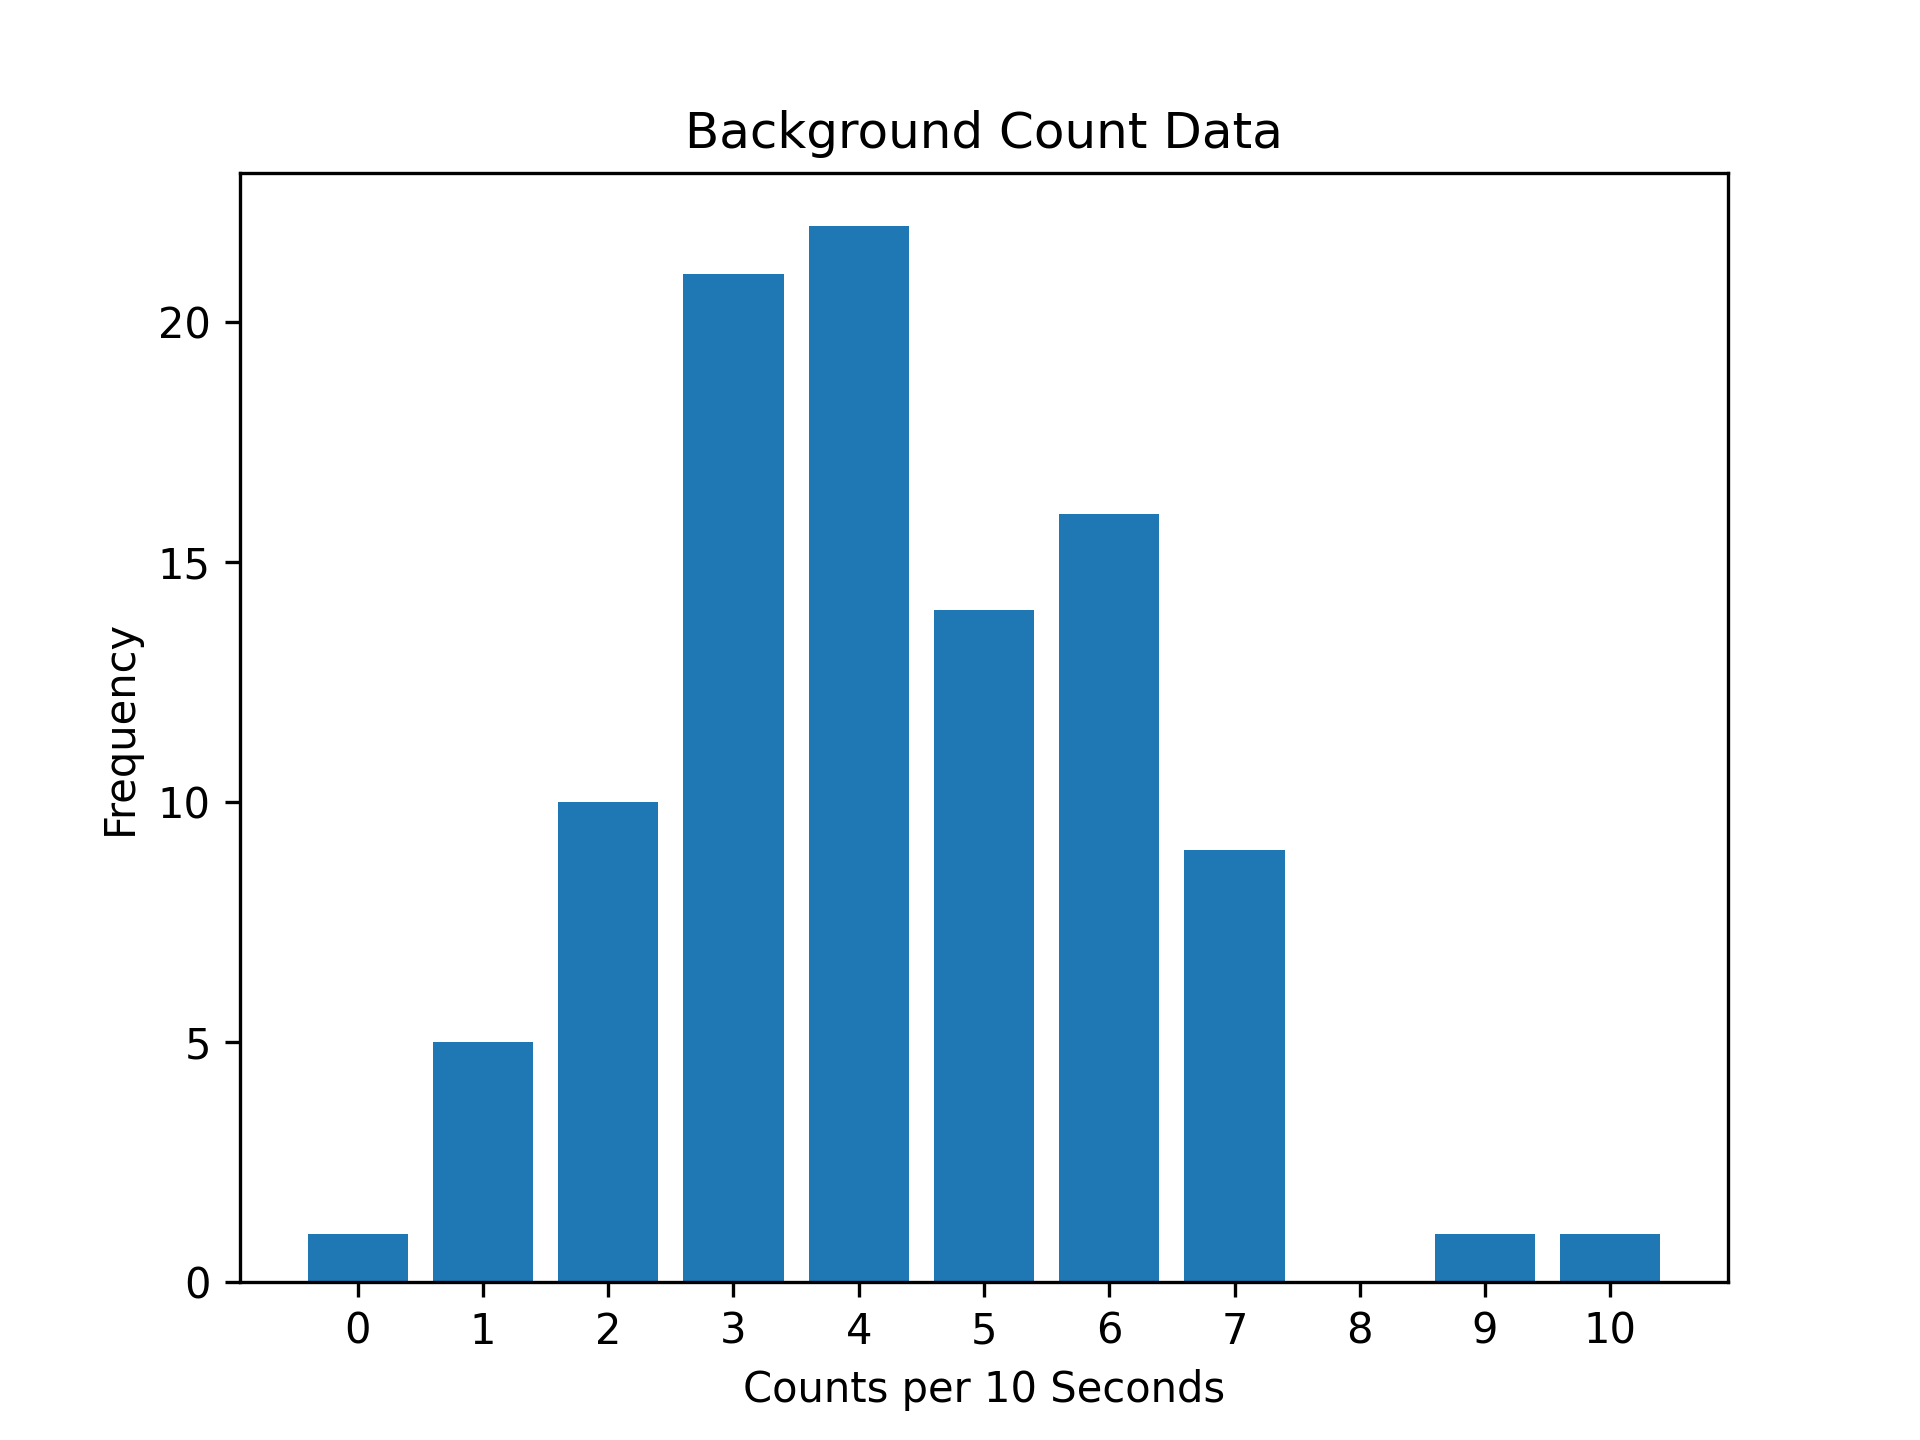
\includegraphics[scale=1]{BackgroundCountHist10sec.png}
	\caption{Count distributions over intervals of 10 seconds for the background measurement.}
\end{figure}

\begin{figure}[H]
	\centering
	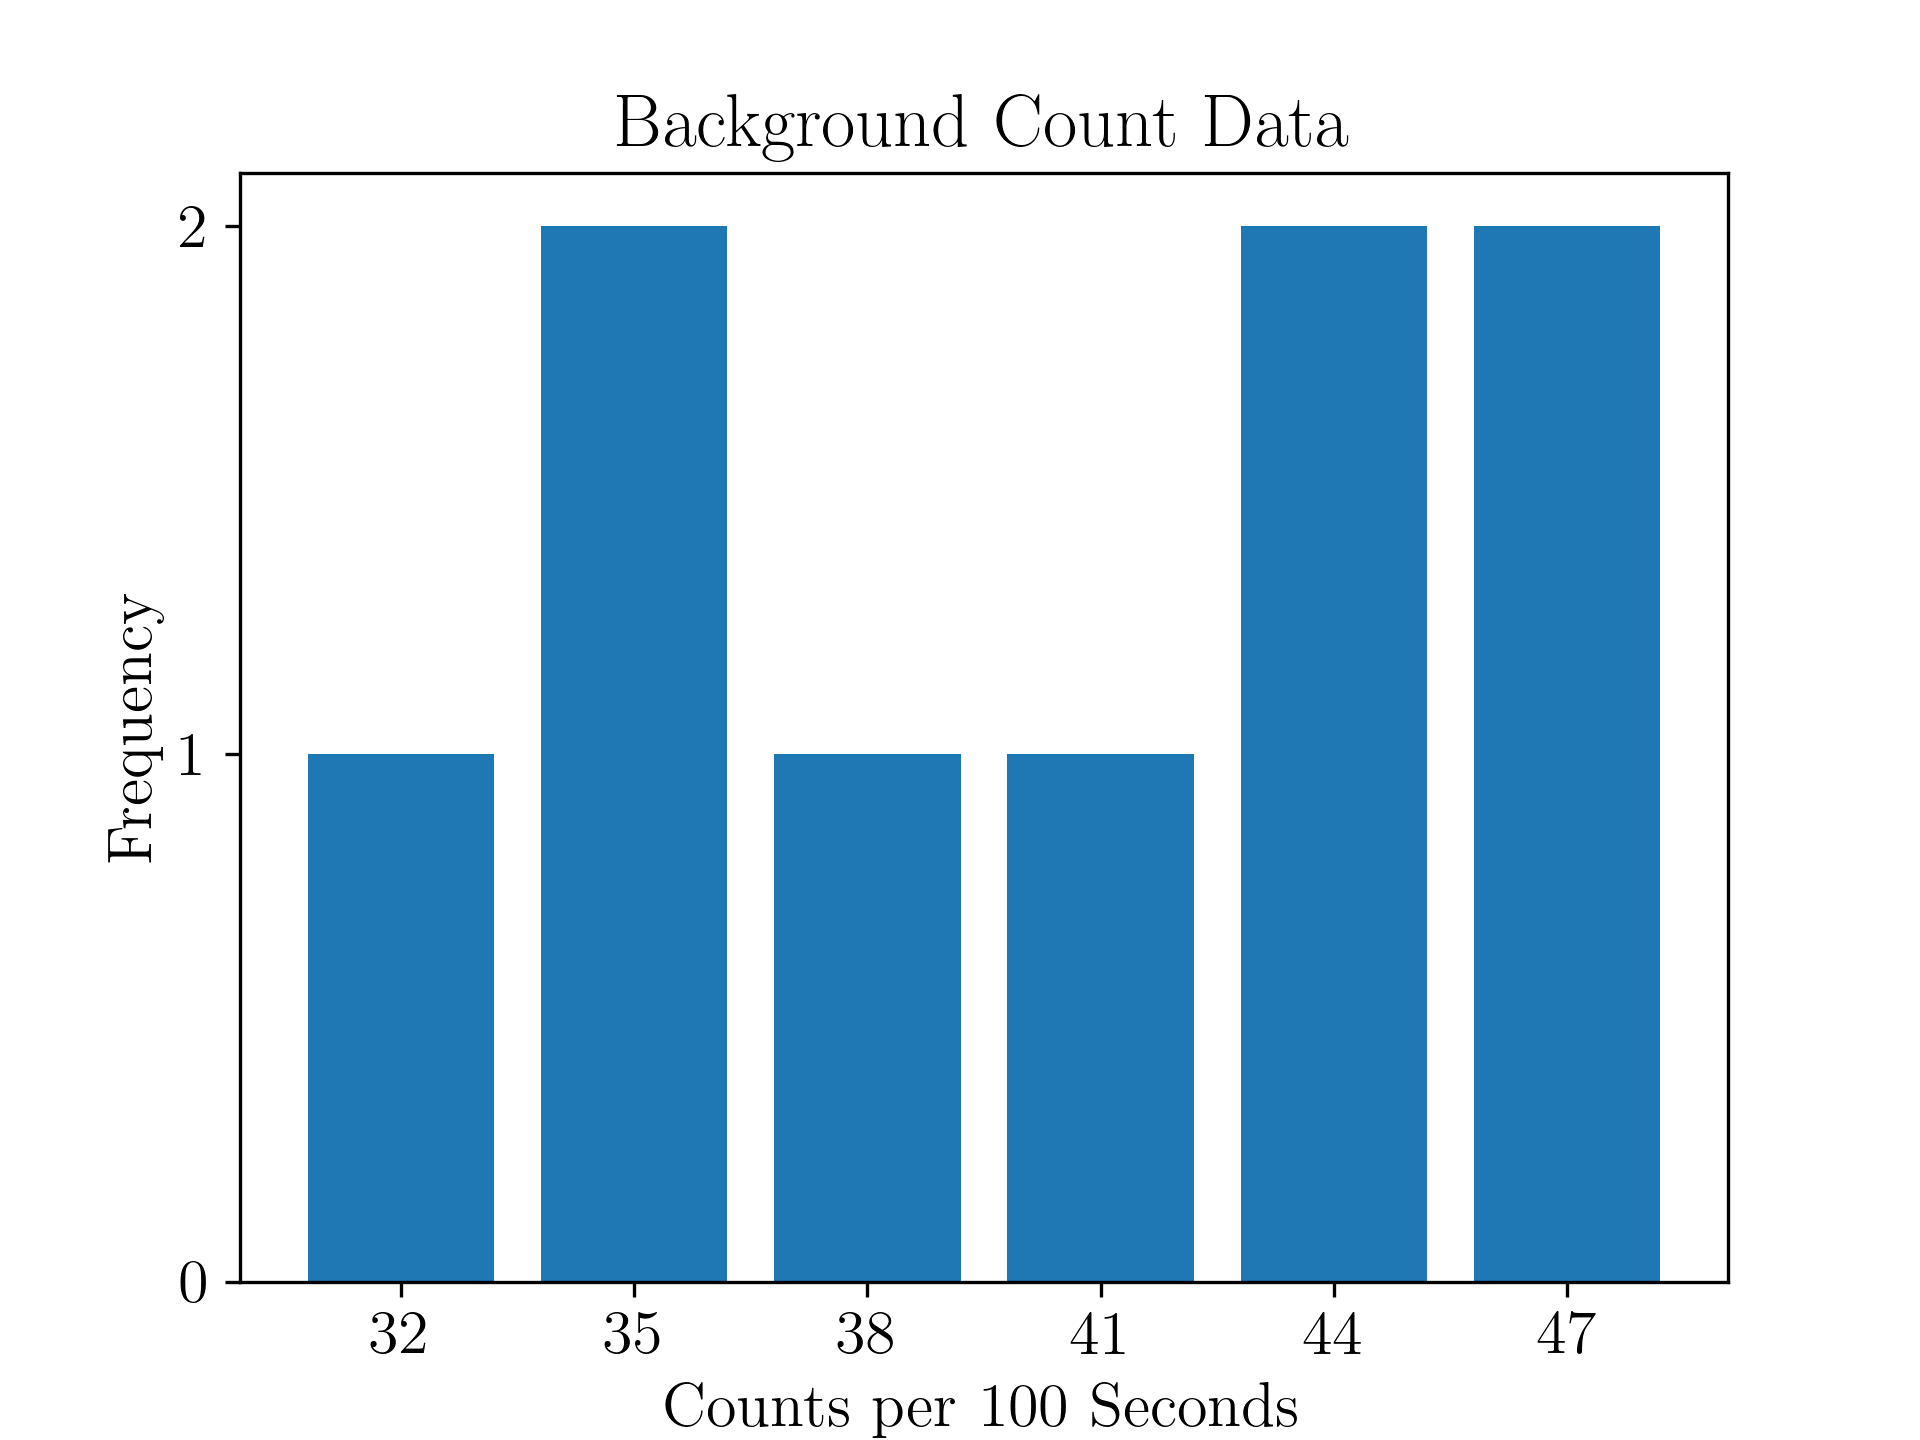
\includegraphics[scale=1]{BackgroundCountHist100sec.png}
	\caption{Count distributions over intervals of 100 seconds for the background measurement.}
\end{figure}

\begin{table}[H]
    \centering
    \captionof{table}{Count and count rate data for the $^{60}$Co shielding experiment} \label{tab:at} 
    \begin{tabular}{ccccc}
\toprule
 d (mm) &  Total Counts &  Total Counts Std. &  Count Rate (Bq) &  Count Rate Std. (Bq) \\
\midrule
 0.0000 &       29669 &         200 &        19.8 &              0.1 \\
 1.6256 &       22194 &         100 &        14.8 &              0.1 \\
 3.1750 &       20293 &         100 &        13.5 &              0.1 \\
 6.3500 &       17420 &         100 &        11.6 &              0.09 \\
\bottomrule
\end{tabular}

\end{table}

\begin{figure}[H]
	\centering
	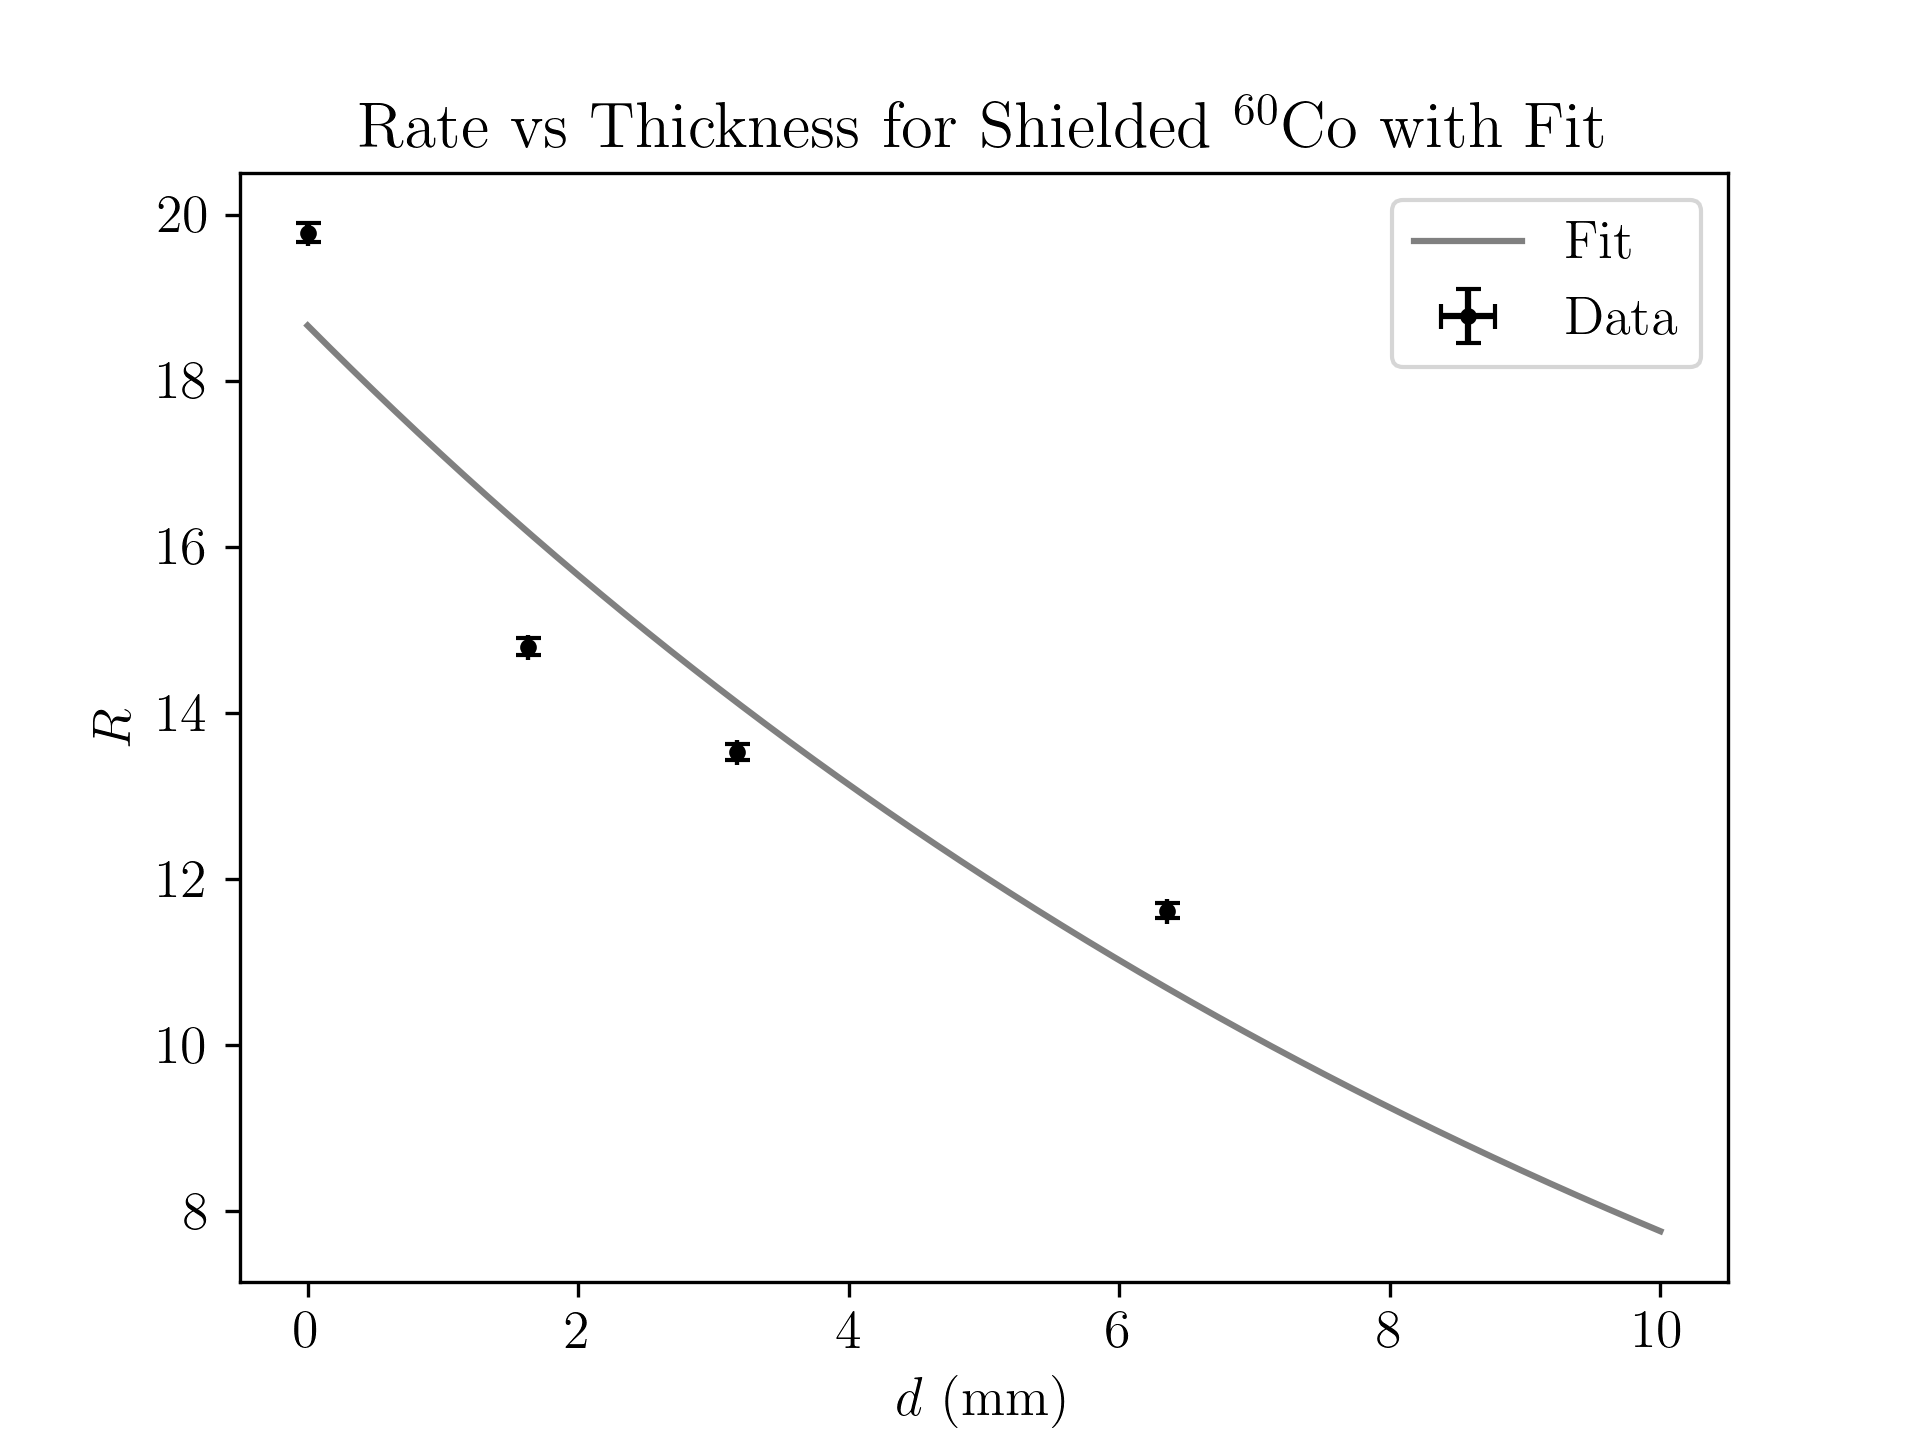
\includegraphics[scale=1]{co60_rate_vs_thickness_fit.png}
	\caption{Rate (Bq) vs shielding thickness (mm) for the shielding experiment using $^{60}$Co. Fitted using the equation $R = R_0 e^{-d/d_0})$, resulting in $R_0 = 18.663 \pm 0.3245$ Bq and $d_0 = 11.387 \pm 0.801$ mm.}
\end{figure}



